\section{Numerische Lösung linearer Gleichungssysteme}
Bei numerischen Berechnungen spielen lineare Gleichungssysteme der Form \textbf{Ax}=\textbf{y} oft eine überaus wichtige Rolle. Daher ist es sinnvoll und von Nöten effiziente Lösungsverfahren für diese Gleichungssysteme zu entwickeln und anzuwenden. In diesem Abschnitt werden verschiedene Verfahren in Octave implementiert und an beispielhaften Gleichungssystemen getestet und gegeneinander verglichen.\\ \\
Zunächst wird eine vorgegebene quadratische Matrix betrachtet. Mit Hilfe des Befehls \texttt{spy} lassen sich Matrizen in Octave graphisch darstellen. In Abb. \ref{fig:bspMat} ist diese Grafik zu sehen, die blauen Punkte in dem Plot sind Einträge, die ungleich null sind. Zählt man diese mit dem Befehl \texttt{nnz} findet man heraus, dass 3.678 der 158.404 Einträge ungleich null sind. Weiterhin lässt sich aus der Abbildung und der Darstellung der Werte in Octave herausfinden, dass es sich um eine symmetrische Matrix handelt, das heißt die Einträge der Matrix sind spiegelsymmetrisch bezüglich der Hauptdiagonalen. \\ \\
\begin{figure}[h]
	\begin{subfigure}[c]{.48\textwidth}
		\centering
		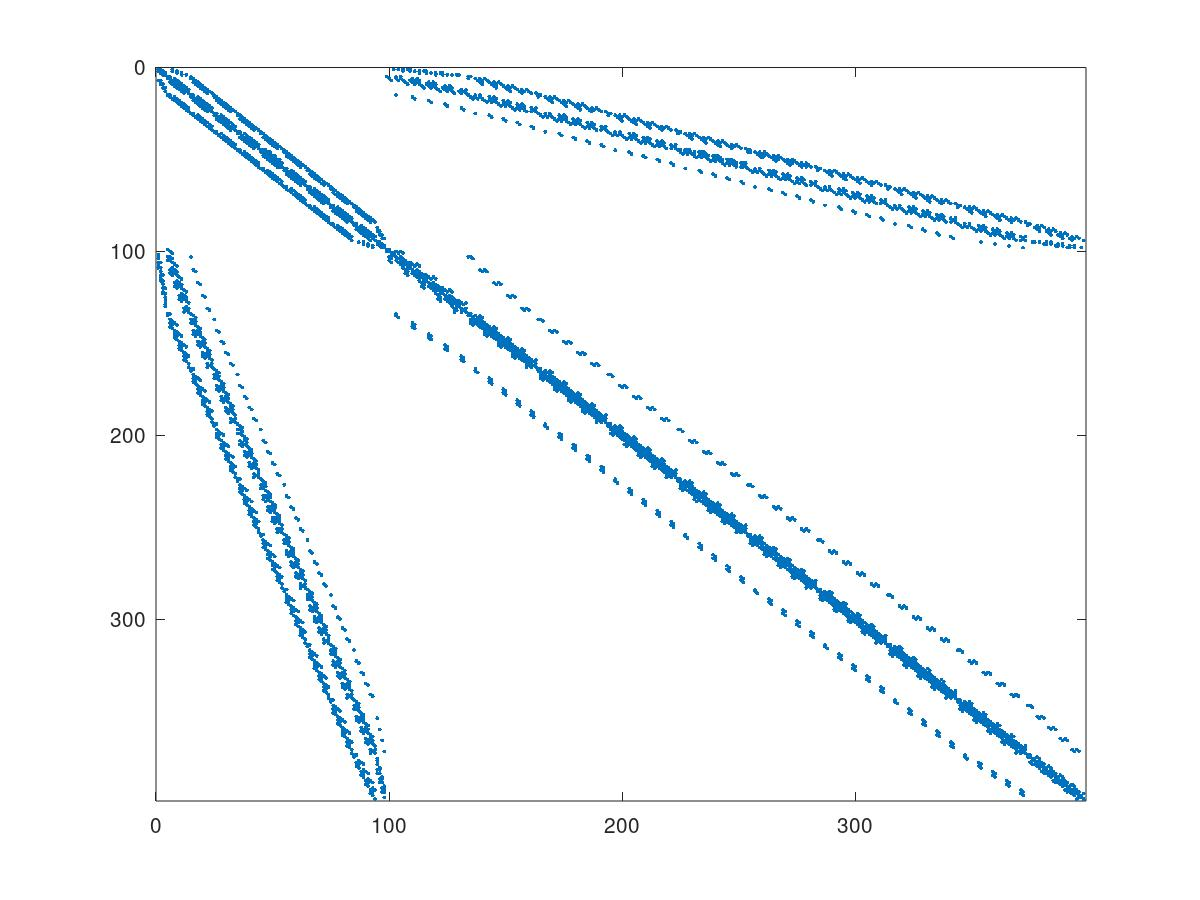
\includegraphics[width=\textwidth]{data/MatrixBsp}
		\subcaption{Graphische Darstellung der mit Octave eingelesene Beispielmatrix}
		\label{fig:bspMat}
	\end{subfigure}
	\begin{subfigure}[c]{.48\textwidth}
		\centering
		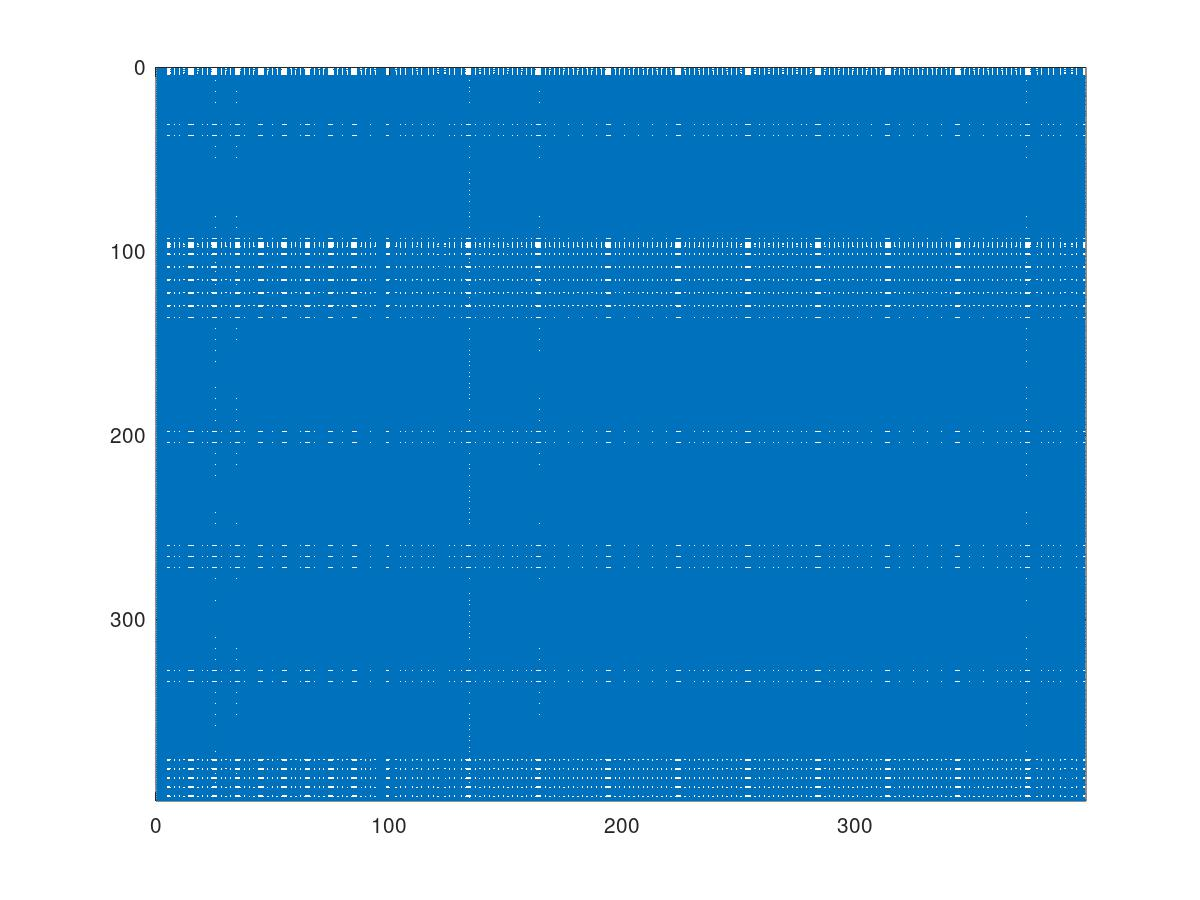
\includegraphics[width=\textwidth]{data/MatrixInv}
		\subcaption{Berechnete Inverse der eingelesenen Matrix}
		\label{fig:inv}\vspace{12pt}
	\end{subfigure}
	\caption{Graphische Darstellung von Matrizen, die blauen Punkte stellen Einträge dar, die ungleich null sind}
\end{figure} \\ 
Nun soll ein erstes Lösungsverfahren in Octave implementiert werden. Das \textsc{Gauss
'sche}-Eliminationsverfahren wurde in Listing \ref{lst:Elim} implementiert. Die Routine \texttt{gaussElim} erhält einen stehenden Vektor \textbf{b} mit Länge $n$ und eine quadratische Matrix \textbf{A} der Größe $n \times n$. Die Rückgabe ist ein Vektor \textbf{x} mit Länge $n$, der die berechneten Lösungen $x_{1}, \dots, x_{n}$ des linearen Gleichungssystems enthält.\\ \\
Zunächst wird \texttt{n}, also die Größe der Matrix bestimmt, daraufhin wird der Ergebnisvektor \textbf{x} mit entsprechender Länge erzeugt. In Zeile 4 und 5 werden zwei Laufvariablen initialisiert, \texttt{j} läuft hierbei über die Spalten, \texttt{i} über die Zeilen. Das Ziel des Algorithmus ist es schrittweise aus der übergebenen Matrix eine untere Dreiecksmatrix zu erstellen. Hierzu werden sogenannte Eliminationsfaktoren bestimmt, siehe Listing \ref{lst:Elim} Zeile 6. Mit Hilfe einer weiteren Laufvariable \texttt{k}, die über die Spalten von \texttt{j} bis \texttt{n} läuft. In der Schleife, Zeile 7 bis 9, werden Zeilenadditionen durchgeführt, um so Spalte für Spalte Nulleinträge zu erzeugen. Auch der Vektor \textbf{b} wird entsprechend angepasst. \\
In den Zeilen 14 bis 17 wird das Gleichungssystem final gelöst, die einzelnen $x_{1}, \dots, x_{n}$ werden von unten nach oben mit Hilfe der Matrix und dem Vektor \textbf{b} berechnet.  \\
Durch die drei ineinander geschachtelten For-Schleifen in den Zeilen 4 bis 12 erhalten wir eine kubische Anzahl an Rechenschritten, $n^{3}-n^{2}$, Zeile 14 bis 17 führen zu einem zusätzlichen Rechenaufwand von $n^{2}-n$, daraus ergibt sich die Abschätzung $\mathcal{O}(n^{3})$.
\lstinputlisting[label=lst:Elim,numbers=left,frame=single]{data/gaussElim.m} 
Lineare Gleichungssysteme lassen sich auch mit Hilfe der Inversen einer Matrix bestimmen. In Octave geht dies mit dem Befehl \texttt{inv(A)}. Wie aus Abbildung \ref{fig:inv}, verglichen mit Abbildung \ref{fig:bspMat}, hervorgeht, hat die Invertierte Matrix deutlich mehr Einträge, die ungleich null sind. Die Berechnung der Inversen benötigt sehr viel Arbeitsspeicher und es werden deutlich mehr Rechenoperationen ausgeführt, um die Lösungen zu berechnen.\\ \\

%%%%%%%%%%%%%%%%%%%%%%%%% Aufgabenteil d %%%%%%%%%%%%%%%%%%%%%%%%%%%%
Eine weitere Methode mit der lineare Gleichungssysteme effizient berechnet werden können ist die LUPQ-Zerlegung. Bei der LUPQ-Zerlegung wird die Matrix \textbf{A} mit Hilfe des bereits vorgestellten \textsc{Gauss'schen}-Eliminationsverfahren in eine obere und eine untere Dreiecksmatrizen aufgeteilt, es gilt $\textbf{A} = \textbf{L} \textbf{U}$. Mit Hilfe von Vorwärts-/Rückwärtseinsetzen lässt sich nun das Gleichungssystem lösen. Zum Lösen wird zunächst vorwärts $$ \textbf{Ly} = \textbf{b}$$ eingesetzt und anschließend rückwärts $$ \textbf{Ux} = \textbf{y}$$ berechnet. Zum berechnen unterschiedlicher Seiten \textbf{b} muss die Matrix nicht neu zerlegt, sondern nur das Vorwärts-/Rückwärtseinsetzen betrachtet werden. Auch dieses Verfahren ist in Octave bereits vorimplementiert und lässt sich mit dem Befehl \texttt{lu(A)} aufrufen. Es ergeben sich bei dieser Methode Unterschiede, die durch die Anzahl der zur Verfügung gestellten Variable in denen die Lösung gespeichert werden soll, hervorgerufen werden.\\
Gibt man der Methode zwei Variablen zum Speichern der Ergebnisse vor, so entsteht nicht wie erwartet eine obere und eine untere Dreiecksmatrix, sondern die in Abbildung \ref{fig:LLU} zu sehende Matrix \textbf{L} und die in Abb. \ref{fig:ULU} Matrix \textbf{U}. Stellt man der Routine vier Variablen \texttt{[L, U, P, Q]} zum Speichern zur Verfügung so entsteht wie in Abb. \ref{fig:LLUPQ} und \ref{fig:ULUPQ} zu sehen ist jeweils eine obere und untere Dreiecks Matrix. Zudem haben diese Matrizen deutlich weniger Einträge. Bei \textbf{P} und \textbf{Q} handelt es sich um Permutationsmatrizen. Mit diesen werden Zeilen und Spalten der Ausgangsmatrix \textbf{A} vertauscht, um zu kleine Pivot Elemente, die zu großen Rundungsfehlern führen können, zu verhindern und zu garantieren, dass die Zerlegung in eine obere und untere Dreiecksmatrix möglich ist. 

\begin{figure}[h!]
	\centering
	\begin{subfigure}[h]{.48\textwidth}
		\centering
		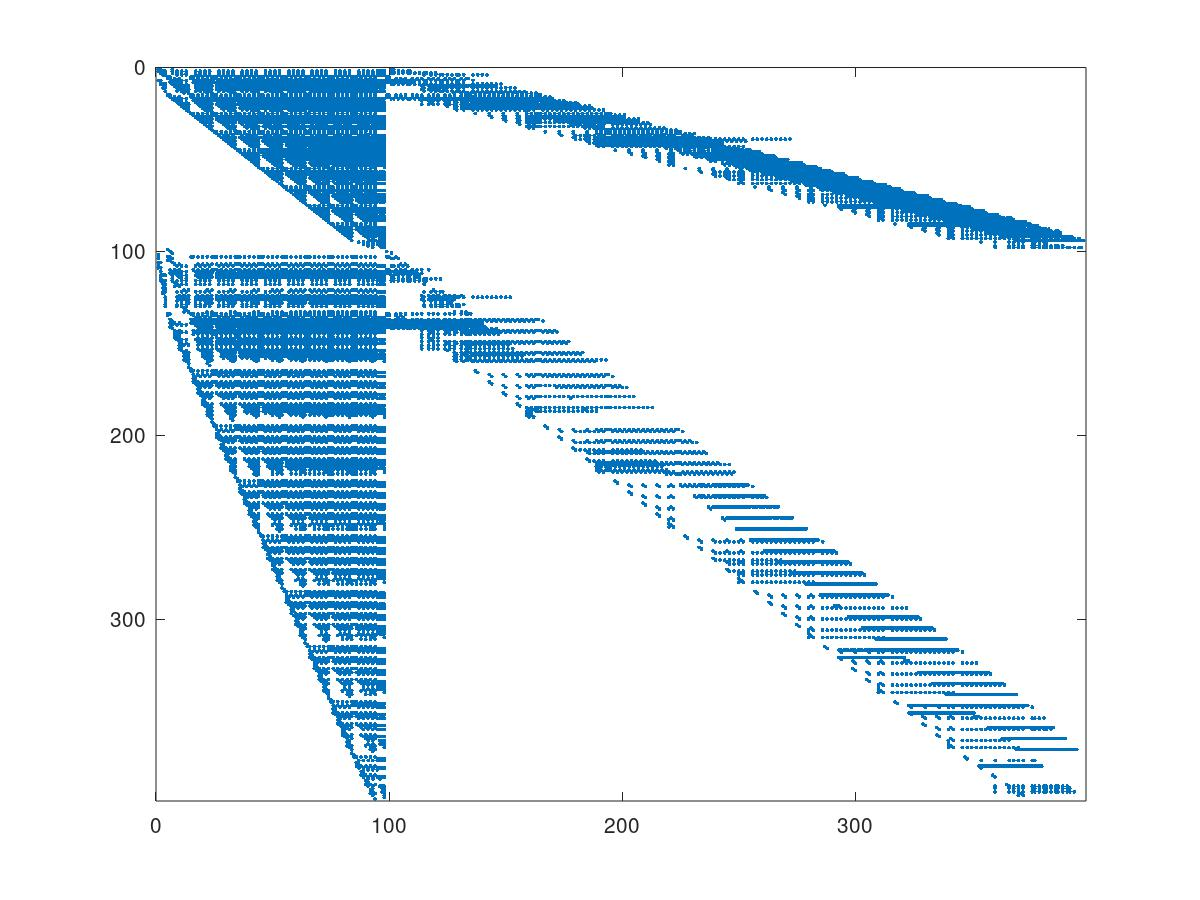
\includegraphics[width=\textwidth]{data/LLU}
		\subcaption{Matrix \textbf{L} nach LU-Zerlegung}
		\label{fig:LLU}
	\end{subfigure}
	\begin{subfigure}[h]{.48\textwidth}
		\centering
		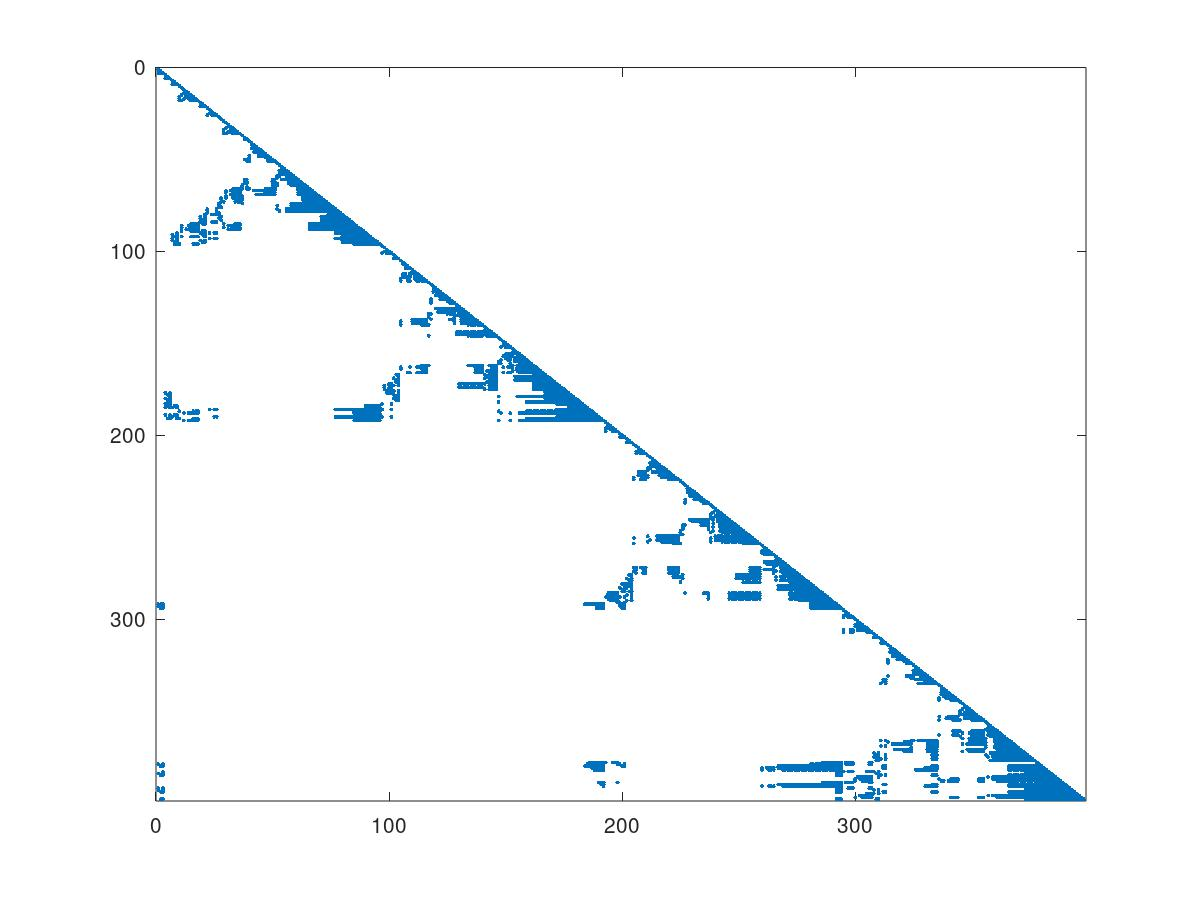
\includegraphics[width=\textwidth]{data/LLUPQ}
		\subcaption{Matrix \textbf{L} nach LUPQ-Zerlegung}
		\label{fig:LLUPQ}
	\end{subfigure}
	\begin{subfigure}[h]{.48\textwidth}
		\centering
		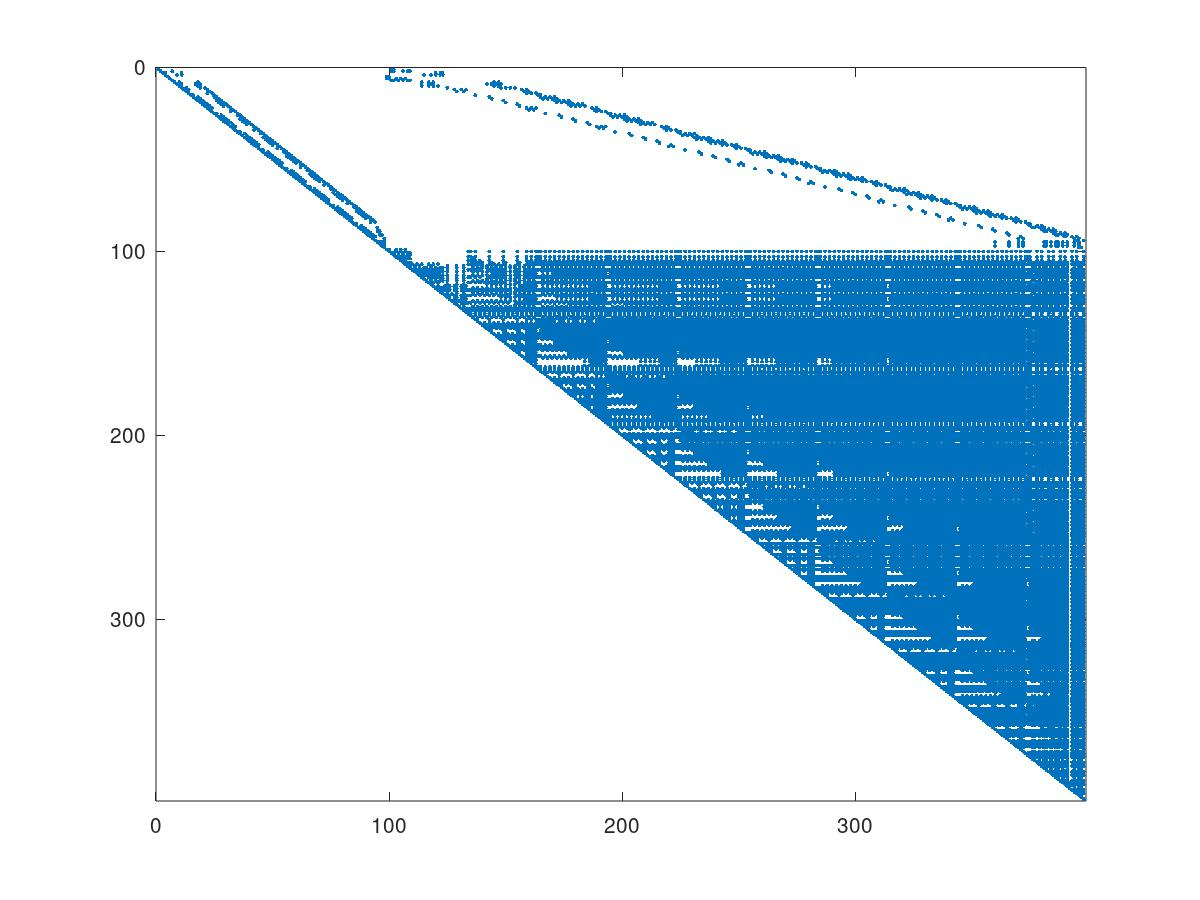
\includegraphics[width=\textwidth]{data/ULU}
		\subcaption{Matrix \textbf{U} nach LU-Zerlegung}
		\label{fig:ULU}
	\end{subfigure}
	\begin{subfigure}[h]{.48\textwidth}
		\centering
		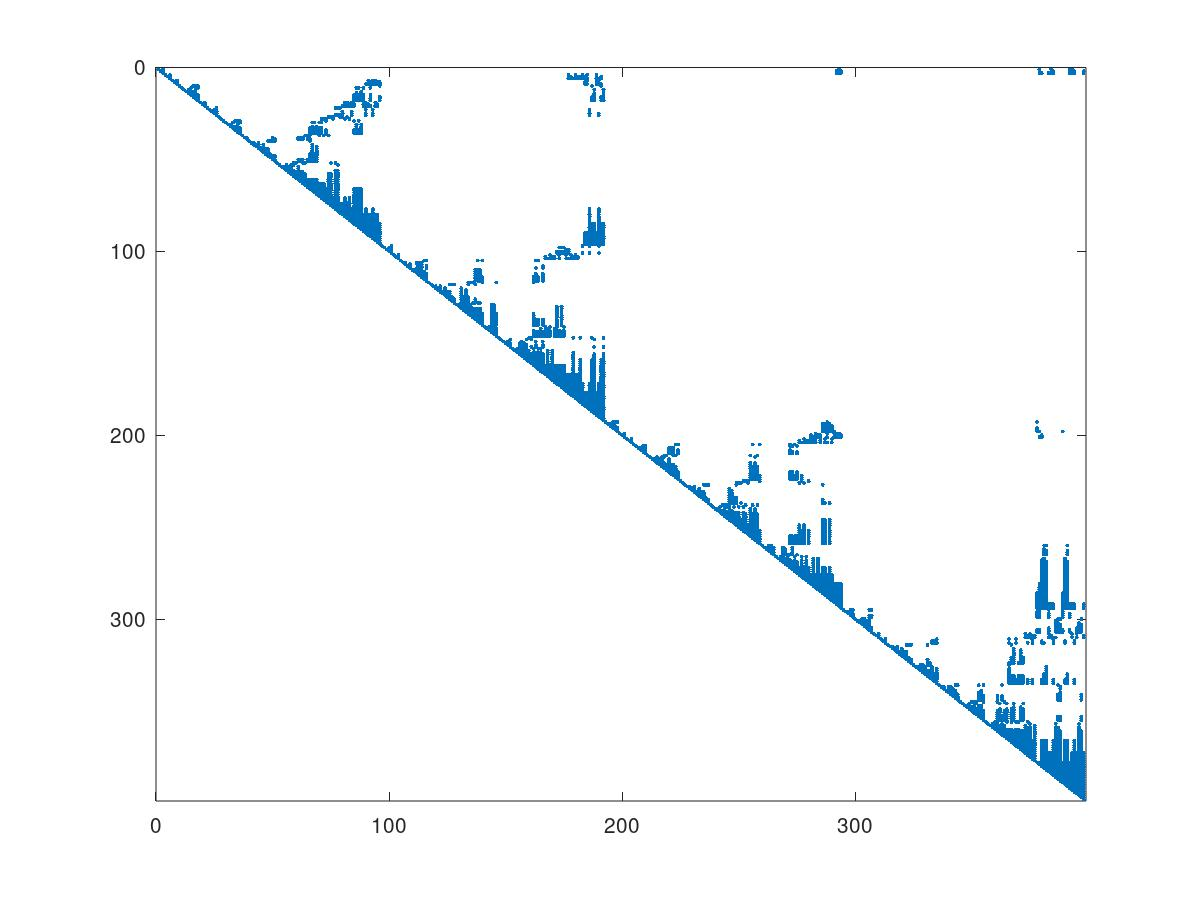
\includegraphics[width=\textwidth,]{data/ULUPQ}
		\subcaption{Matrix \textbf{U} nach LUPQ-Zerlegung}
		\label{fig:ULUPQ}
	\end{subfigure}%\hspace{40pt}
\caption{Darstellung der unterschiedlichen Matrizen, die abhängig der zur Verfügung gestellten Lösungsvariablen entstehen}
\end{figure}

Um den zeitlichen Aufwand der einzelnen Lösungsverfahren besser vergleichen zu können wird im Folgenden eine Messung der benötigten Rechenzeit in Octave durchgeführt und beschrieben. Die zu vergleichenden Lösungsverfahren zur Berechnung linearer Gleichungssysteme sind die LUPQ-Zerlegung, Lösung mit Hilfe des Backslash-Operators und die Berechnung mit der Inversen.\\ \\
Verschiedene tridiagonale Testmatrizen \textbf{A} der Größe $n \times n$ mit $n \in [500, 1000, 2000, 4000, 8000]$ haben jeweils 10 unterschiedliche, zufällige Seiten \textbf{b} zugewiesen bekommen. Die Zeit zur Berechnung jeder einzelnen Seite wurde gespeichert, die Berechnung der Inversen bzw. der LUPQ Zerlegung fließt nur bei der ersten Berechnung mit in die Rechenzeit ein. \\
Die Rechenzeit, die benötigt wurde um alle 10 Seiten zu berechnen wurde schließlich durch 10 geteilt, um eine durchschnittliche Rechenzeit zu erhalten. Die Ergebnisse wurden abschließend auf einem doppelt logarithmischen Koordinatensystem geplottet, wobei die x-Achse die Größe $n$ der Matrix ist und die y-Achse die zur Berechnung einer Seite benötigte Rechenzeit.
\begin{figure}
	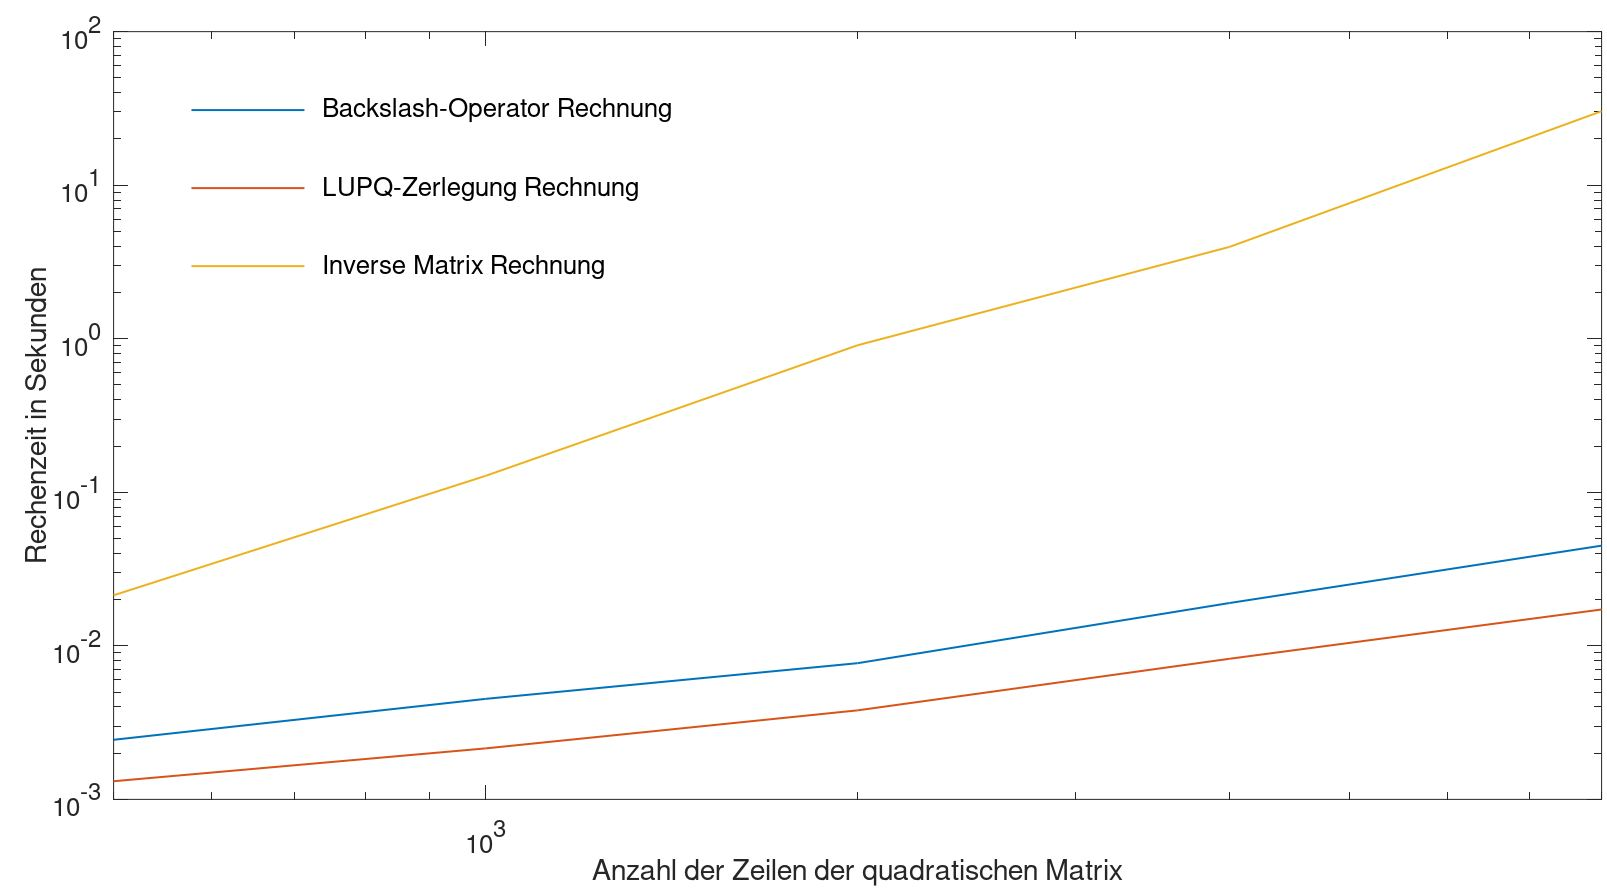
\includegraphics[width=\textwidth]{data/LaufzeitPlot}
	\caption{Graphische Darstellung der Rechenzeit, die unterschiedliche Lösungsverfahren zum Lösen linearer Gleichungen benötigen}
	\label{fig:Laufzeit}
\end{figure}
\\ \\
Wie aus Abbildung \ref{fig:Laufzeit} erkenntlich ist, benötigt die LUPQ-Zerlegung die geringste Zeit, um die Gleichungssysteme zu lösen. Der Backslash Operator benötigt mehr Zeit, ist aber, verglichen zur Berechnung mit Hilfe der Inversen, immer noch effizient. 